\newsavebox{\FOnegraphicbox}
\begingroup
\makeatletter
\let\FOneoriginalendfloatbox\@endfloatbox
\def\@endfloatbox{\FOneoriginalendfloatbox
\typeout{FONE-FLOAT-HEIGHT=\the\ht\@currbox}
\typeout{FONE-FLOAT-DEPTH=\the\dp\@currbox}}
\makeatother
\begin{figure*}[t]
  \centering
  \sbox{\FOnegraphicbox}{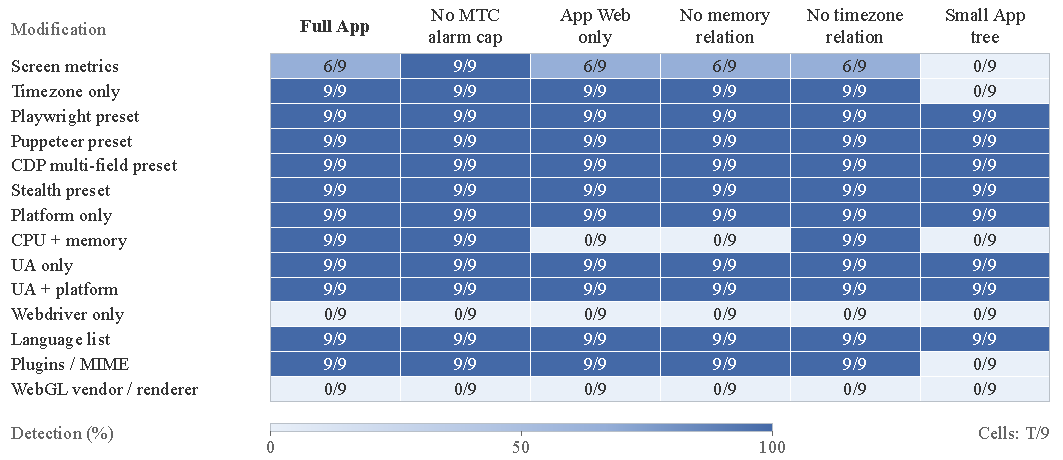
\includegraphics[width=\textwidth]{figures/F01_main.pdf}}
\typeout{FONE-TEXTWIDTH=\the\textwidth}
\typeout{FONE-TEXTHEIGHT=\the\textheight}
\typeout{FONE-GRAPHIC-WIDTH=\the\wd\FOnegraphicbox}
\typeout{FONE-GRAPHIC-HEIGHT=\the\ht\FOnegraphicbox}
\typeout{FONE-GRAPHIC-DEPTH=\the\dp\FOnegraphicbox}
\usebox{\FOnegraphicbox}
  \caption{Detection across 14 App modification configurations and six methods from saved evaluations. Cells show alarm detections T/N (N=9 per configuration); color encodes detection proportion on a shared 0-100\% scale. Full App is the current App-only detector, excluding standalone-browser C1, new Host geometry, and unintegrated resource conditions. Rule methods use RETENTION outputs; the small App tree uses FITTED outputs. Normal-record costs are reported in the companion normal-results analysis; removing the MTC alarm cap must not be judged superior from this heatmap alone. These materials have a development-use history and do not constitute a new blind test.}
  \Description{Fourteen modification configurations in the original order and six App methods. Every cell shows the saved alarm count out of nine. A shared blue scale encodes detection proportion. Zero detections and partial detections remain explicit.}
  \label{fig:hybridguard-overview}\label{fig:app-modification-detection}
\end{figure*}
\endgroup
